\subsection{Results}

In this section, we describe findings on how participants verified the LLM-based evaluations (\S\ref{sec:rq1}, RQ1), identified issues with the task LLM's outputs (\S\ref{sec:rq2}, RQ2), revised criteria to correct the evaluations (\S\ref{sec:rq3}, RQ3), and explored fragment-level functions for multiple criteria (\S\ref{sec:rq4}, RQ4).

\begin{figure*}[b]
    \centering
    \includegraphics[width=1.00\textwidth]{figures/results_issues.pdf}
    \caption{Comparison of results across conditions for the issues identified for the task LLM's outputs (left) and LLM evaluations (right). Results present the average number of issues identified, and the distribution of participants' ratings regarding the importance, comprehensiveness, and actionability of the issues (*:p<.05, **:p<.01, error bars indicate one standard deviation).}
    \Description{This figure compares the Fragmented and Holistic conditions in two sections: output-related issues and evaluation-related issues. Each section includes a bar chart showing the average number of identified issues with standard deviation, and stacked bar charts showing the distribution of participant’s 7-point Likert ratings for importance, comprehensiveness, and actionability of the identified issues. Participants identified significantly more output-related issues in the Fragmented condition (M=3.40) than in the Holistic condition (M=2.30). Ratings also suggest that output-related issues in the Fragmented condition were seen as more actionable.}
    \label{fig:results_issues}
\end{figure*}

\subsubsection{Verifying Evaluations}
\label{sec:rq1}

Participants identified significantly more issues with the LLM-based evaluations in the \treatment{} condition \stats{3.40}{1.58}{2.30}{1.42}{t}{-2.40}{=0.04} (Fig.~\ref{fig:results_issues}).
Participants attributed this to how it was easier to read and understand the fragment evaluations.
Instead of reading entire outputs and overall justifications as in the \control{} condition, participants only had to review individual fragments, their function labels, and their shorter justifications in the \treatment{} condition.
P1 noted that \myquote{the range of text that I had to read was smaller so it was less time-consuming to interpret each data point.}
As a result, P5 mentioned, \myquote{I read each evaluation more carefully and I was able to concentrate on each one more.}

Furthermore, participants mentioned how, as it was easier to verify each individual evaluation, it was also easier to verify their consistency.
P3 explained, \myquote{As [each output's] evaluation is split [into multiple fragment-level functions], I could see multiple evaluations [for fragments from different outputs] together and easily compare them, so I tended to focus on that.}
In contrast, with the \control{} condition, P4 mentioned how \myquote{while I could see general trends in the evaluations, I could not directly compare them} due to the amount of text (i.e., outputs and overall justifications) to compare and reason about.
Most participants (7/10) recognized the importance of identifying when the LLM-based evaluator is inconsistent, and explicitly focused on verifying this.

As participants' ability to verify the evaluations differed in each condition, their trust and reliance on these evaluations also differed.
As participants could more \myquote{confidently} (P1) verify evaluations in \treatment{}, they mentioned how they could judge their trust in the evaluations more carefully.
P7 mentioned: \myquote{it's not that I have more trust but instead that it is easier to verify my trust.}
Three participants explained how they \myquote{empathized} with the LLM evaluator---explaining that they may not agree with its evaluation but understood why it returned such an evaluation.
As a result, participants mentioned how they were able to develop more \textit{informed trust} about the LLM evaluator by identifying the fragment-level functions for which they agreed with the evaluator and when it is consistent or not.
P5 explained: \myquote{I was wondering whether the evaluator had a bias when evaluating [a certain function] so I looked at these [clusters] more. My conclusion was that it seems like the LLM evaluator considers the aspect as negative most of the times, but there is a slight fluctuation.}

On the other hand, participants struggled to develop more \textit{informed trust} in the \control{} condition.
Some participants mentioned how they trusted the holistic evaluations despite not carefully inspecting them.
For example, P7 mentioned that \myquote{if an output got a score of 100\% and the [one-line justification summary] seems to make sense, I just move on}.
Others mentioned not trusting the holistic evaluations at all as they could not confidently verify them: \myquote{I didn't look at the summary or justification at all because I just didn't have trust in them} (P5).
Interestingly, regardless of their trust in the evaluations, most participants (7/10) mentioned relying on the evaluation scores to decide which outputs to explore---often focusing on \textit{extreme} cases (i.e., scores of 100\% or 0\%)---even without fully understanding why those outputs received those scores.

\subsubsection{Identifying Model Issues}
\label{sec:rq2}

Overall, participants identified a similar number of issues in the task LLM's outputs in both conditions \stats{2.70}{0.82}{3.60}{2.12}{w}{4.00}{=0.09}.
However, participants rated that they were significantly more confident that they could act on and resolve the issues identified with the \treatment{} condition \stats{5.10}{1.20}{3.00}{1.85}{w}{0.00}{=0.04} (Fig.~\ref{fig:results_issues}).

Participants attributed this to their trust and dependency in the LLM-based evaluations.
As participants developed more informed trust regarding the evaluations in the \treatment{} condition, they used the evaluations as guidance when determining the quality of the outputs---inspecting outputs \myquote{piece-by-piece} (P1) and \myquote{more specifically} (P2).
Furthermore, participants mentioned how the \treatment{} condition allowed them to explore output issues from a \myquote{wider perspective} (P5) by exploring similar issues across outputs and considering more \myquote{diverse characteristics} (P6) regarding the criterion.

In contrast, in the \control{} condition, participants could not adequately gauge their trust in the evaluations, so they would frequently manually inspected the outputs themselves without relying on the LLM-based evaluations.
For example, P3 mentioned: \myquote{In the [\control{} condition], I had to read all of the [output] and also the justification, so I focused only on the [output] and tended to not look at the justification.}
By manually reviewing the outputs themselves, participants not only lost efficiency benefits from the LLM-based evaluations but they also tended to focus on more abstract or surface-level issues regarding the model outputs (e.g., overall writing quality, coherency, logic).
As they were less concrete, P8 explained that these broader issues could be more challenging to resolve: \myquote{The issues I identified seem more related to the limitations of the model itself [...] No matter what feedback I give, it will be difficult to resolve these.}
This is also reflected in the interaction logs, where participants in \control{} frequently viewed each output in detail \stats{20.92}{9.35}{33.91}{13.32}{w}{0.00}{<0.001}, while participants in \treatment{} interacted more frequently with the Explore Tab and Map Visualization, selecting and navigating between data points \stats{59.25}{27.89}{33.92}{20.69}{w}{9.00}{=0.02}.

Although the \treatment{} condition helped participants find more actionable issues, they also mentioned how it had limitations.
Specifically, participants mentioned how they tended to lose sight of the \myquote{bigger picture} (P2), referring to the overall qualities of outputs (e.g., structure, coherency, and context).
As a result, participants mentioned how they appreciated the \control{} condition as it allowed them to compare these holistic aspects of outputs.
In fact, after exploring fragment-level functions, participants in the \treatment{} condition frequently went back to the Database Tab as this was the only tab that allowed them to look at outputs one-by-one and compare them.

\subsubsection{Correcting Evaluations}
\label{sec:rq3}

We observed substantial differences in the difficulty of correcting the given evaluation issues across study tasks. 
Rather than overall comparisons between conditions, we report success rates for each task-condition pair to provide descriptive insights, without statistical tests due to limited sample size (N=5 per pair).
In the advertisement task, success rates in correcting the evaluation issues were higher in the \treatment{} condition ($\text{\treatment{}} = 77.0\% \pm 7.9\%$, $\text{\control{}} = 72.7\% \pm 9.8\%$).
Conversely, in the horror story task, success rates were higher in the \control{} condition ($\text{\treatment{}} = 24.9\% \pm 14.4\%$, $\text{\control{}} = 37.7\% \pm 7.3\%$).

Participants found \treatment{} helpful for skimming through evaluations to identify potential examples for the criteria.
However, for each example, \treatment{} required participants to add the entire fragment that the system extracted, which sometimes spanned multiple sentences.
Due to this, P5 hesitated to add examples in the \treatment{} condition: \myquote{since the whole [fragment] will be considered in future evaluations, I worry that [the evaluator] will interpret it differently.
In contrast, \control{} allowed participants to manually select shorter fragments to add as examples, which they used to precisely select only the most relevant content.}
Qualitative analysis of results indicated that the lower success rate in \treatment{} for the horror story task stemmed from this limitation: automatically extracted fragments contained multiple sentences but participants likely added these as examples due to a short phrase within them.
This suggests the need for a combined approach: fragment evaluations to identify evaluation issues, with the ability to select specific sub-fragments to precisely express intended corrections.

In \treatment{}, participants would verify how adding examples to the criteria corrected and influenced the evaluations by rerunning the evaluations and using the Map Visualization to check how the evaluations changed.
Several participants confirmed that they could see their feedback being incorporated. 
For instance, P9 mentioned \myquote{[newly added examples] seemed to be reflected} after observing that functions close to an example all adopted the same rating.
This illustrates how the \treatment{} condition facilitated participants' iterative refinement of criteria by helping them identify functions to add as examples, steer the evaluations based on those examples, and verify the effects of this steering.

\subsubsection{Exploration with Multiple Criteria}
\label{sec:rq4}

By exploring fragment-level functions for a new criterion (RQ4), participants were able to gain new insights about the outputs and the evaluations.
For example, P7 observed that the fragment \textit{``experience a true `smart life' with it''} in an advertisement was positively rated for \criterion{Emotional Effect}, but negative for \criterion{Call-to-Action} as it only provides an abstract suggestion---highlighting the challenge of satisfying multiple criteria simultaneously and the opportunities for model refinement.
As a result, P7 mentioned how he wanted to\myquote{compare the distribution of evaluations in one cluster with those in a different criterion's cluster.}
P6 explained how they could use these seemingly conflicting evaluations to decide on what outputs to use for \myquote{different use cases and applications}.
P1 also noted that there was a \myquote{hierarchy} between the criteria that helped her gain both a broad and detailed understanding of outputs. 
The criterion \criterion{Keyword Cohesion} (e.g., whether keywords are properly integrated in the horror story) helped her understand the broad alignment of the output's content and its overall flow.
Then, with \criterion{Horror Atmosphere}, she could narrow down to sentence-level stylistic details (e.g., whether sentences effectively evoke a horror atmosphere).

Participants noted that, by surfacing fragment-level functions relevant to each criterion instead of simply providing a score, \sysname{} allowed them to \myquote{more deeply understand and define each criterion} (P4).
P2 mentioned: \myquote{When one doesn't really know what is relevant to a criterion, they could just add an abstract description of the criterion [into the system], and see the LLM evaluations and clusters to learn more and concretize the criterion further.}
P5 also reflected this sentiment: \myquote{[In practice], one needs to revise their evaluation criterion by actually evaluating outputs to see [how they match with the criterion], but it seems like this is already doing all of that for us.}
Participants compared the system to a process like \textit{inductive coding}, where one starts with a broad and abstract criteria and, through the process of reviewing outputs, identifies relevant fine-grained functions that can concretize this criterion.

\begin{figure}[t]
    \centering
    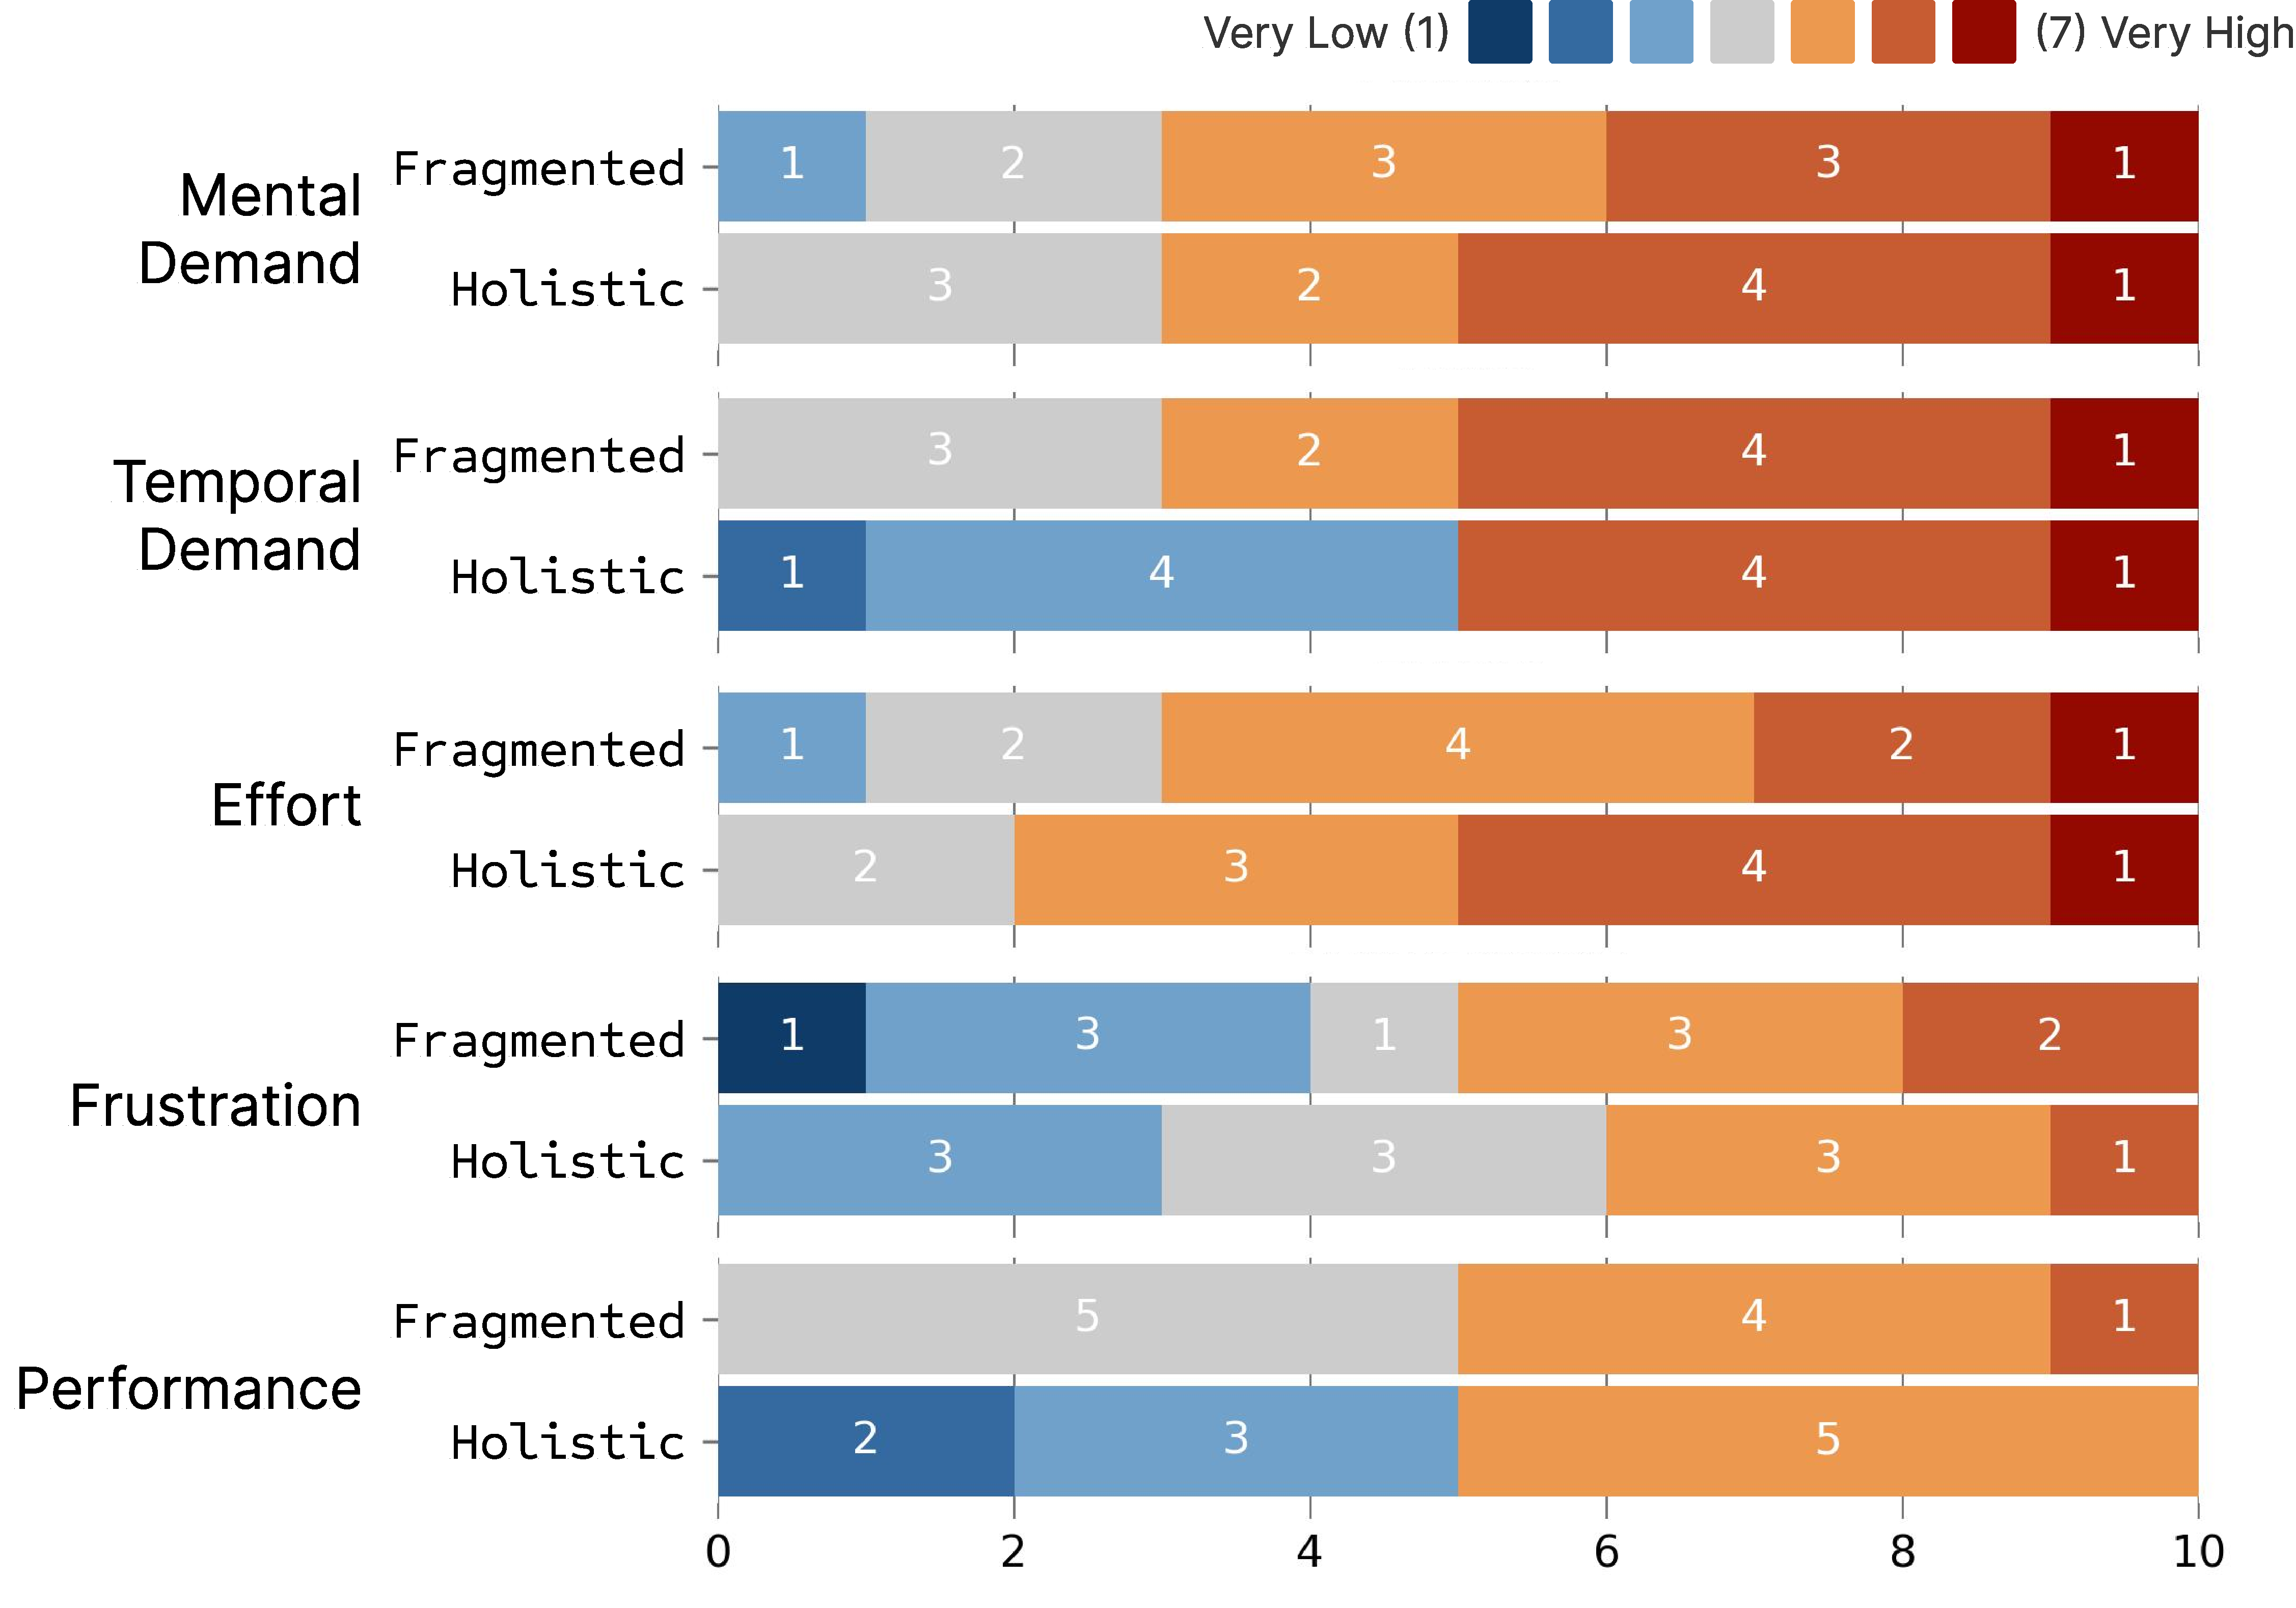
\includegraphics[width=1.0\columnwidth]{figures/results_tlx_twocol.pdf}
    \caption{Distribution of participants’ ratings for perceived workload (i.e., NASA-TLX) show that participants perceived a similar amount of workload in both conditions. In general, participants expressed feeling high workload due to the demands of the study task.}
    \Description{This figure presents the distribution of participants’ ratings for perceived workload across five NASA-TLX dimensions—Mental Demand, Temporal Demand, Effort, Frustration, and Performance—under Fragmented and Holistic conditions. Each bar shows a 7-point Likert scale distribution from Very Low (1, dark blue) to Very High (7, dark red). Overall, participants reported similar workload levels across both conditions, with generally high perceived workload due to the task demands.}
    \label{fig:results_tlx}
\end{figure}

\subsubsection{Perceived Workload}

\autoref{fig:results_tlx} shows that overall perceived workload was similar in both conditions \stats{4.58}{0.43}{4.72}{0.78}{t}{0.51}{=0.62}, which is attributed to how each condition led to different distributions of cognitive effort.
In \treatment{}, verifying the evaluations required less effort which freed participants to compare and explore these evaluations. 
In contrast, \control{} led participants to expend most of their effort into manually reviewing outputs one by one.
Also, while the fragment-level functions supported more fine-grained exploration and analysis, some participants found the number of functions to be overwhelming.
For example, P7 mentioned that \myquote{The [\treatment{}] visualization felt a bit complex and had too many colors, which made it hard to see what information I should focus on. In contrast, the [\control{}] visualization was much easier and didn’t feel tiring to look at.}
